\documentclass[11pt,oneside,letterpaper]{article}

% graphicx package, useful for including eps and pdf graphics
\usepackage{graphicx}
\DeclareGraphicsExtensions{.pdf,.png,.jpg}

% basic packages
\usepackage{color} 
\usepackage{parskip}
\usepackage{float}

% text layout
\usepackage{geometry}
\geometry{textwidth=15cm} % 15.25cm for single-space, 16.25cm for double-space
\geometry{textheight=22cm} % 22cm for single-space, 22.5cm for double-space

% helps to keep figures from being orphaned on a page by themselves
\renewcommand{\topfraction}{0.85}
\renewcommand{\textfraction}{0.1}

% bold the 'Figure #' in the caption and separate it with a period
% Captions will be left justified
\usepackage[labelfont=bf,labelsep=period,font=small]{caption}

% review layout with double-spacing
%\usepackage{setspace} 
%\doublespacing
%\captionsetup{labelfont=bf,labelsep=period,font=doublespacing}

% cite package, to clean up citations in the main text. Do not remove.
\usepackage{cite}
%\renewcommand\citeleft{(}
%\renewcommand\citeright{)}
%\renewcommand\citeform[1]{\textsl{#1}}

% Remove brackets from numbering in list of References
\renewcommand\refname{\large References}
\makeatletter
\renewcommand{\@biblabel}[1]{\quad#1.}
\makeatother

\usepackage{authblk}
\renewcommand\Authands{ \& }
\renewcommand\Authfont{\normalsize \bf}
\renewcommand\Affilfont{\small \normalfont}

% notation
\usepackage{amssymb}
\newcommand{\point}{f_{\scriptscriptstyle \vert}}	% point likelihood
\newcommand{\threshold}{f_{\textstyle \lrcorner}}	% threshold likelihood
\newcommand{\interval}{f_{\sqcup}}					% interval likelihood
\newcommand{\mdssd}{\varphi}						% MDS standard deviation
\newcommand{\diffusionsd}{\sigma}					% Diffusion standard deviation
\newcommand{\tree}{\tau}							% Phylogeny
\newcommand{\vn}{n}									% Number of viruses
\newcommand{\sn}{k}									% Number of sera

% comments
\usepackage{ulem}
\definecolor{purple}{rgb}{0.459,0.109,0.538}
\def\tb#1#2{\sout{#1} \textcolor{purple}{#2}} 
\def\tbc#1{\textcolor{purple}{[#1]}}

%%% TITLE %%%
\title{\vspace{1.0cm} \LARGE \bf Revealing the competitive dynamics of influenza viruses through evolutionary cartography}

\author[1]{Trevor Bedford}
\author[2,3,4]{Marc A. Suchard}
\author[5]{Philippe Lemey}
\author[1]{Gytis Dudas}
\author[6]{Colin Russell}
\author[6,7]{Derek Smith}
\author[1,8]{Andrew Rambaut}

\affil[1]{Institute of Evolutionary Biology, University of Edinburgh, Edinburgh, UK}
\affil[2]{Department of Biomathematics, David Geffen School of Medicine at UCLA, University of California, Los Angeles CA, USA}
\affil[3]{Department of Human Genetics, David Geffen School of Medicine at UCLA, University of California, Los Angeles CA, USA}
\affil[4]{Department of Biostatistics, UCLA School of Public Health, University of California, Los Angeles CA, USA}
\affil[5]{Department of Microbiology and Immunology, Katholieke Universiteit Leuven, Leuven, Belgium}
\affil[6]{Department of Zoology, University of Cambridge, Cambridge, UK.}
\affil[7]{Department of Virology, Erasmus Medical Centre, Rotterdam, Netherlands.}
\affil[8]{Fogarty International Center, National Institutes of Health, Bethesda, MD, USA.}

\date{}

\begin{document}

\maketitle

%%% ABSTRACT %%%

% Abstracts explain to the general reader why the research was done and why the results are important. They should start with some brief BACKGROUND information: a sentence giving a broad introduction to the field comprehensible to the general reader, and then a sentence of more detailed background specific to your study. This should be followed by the RESULTS, or if the paper is more methods/technique oriented an explanation of OBJECTIVES/METHODS and then the RESULTS. The final sentence should outline the main CONCLUSIONS of the study, in terms that will be comprehensible to all our readers. The abstract should be 125 words or less.

\section*{Abstract}

%%% INTRODUCTION %%%
\section*{Introduction}

Seasonal influenza infects between 10\% and 20\% of the human population every year, causing 250,000 to 500,000 deaths annually \cite{flufactsheet}. 
While individuals develop long-lasting immunity to particular influenza strains after infection, antigenic mutations to the influenza virus genome result in proteins that are recognized to a lesser degree by the human immune system, leaving individuals susceptible to future infection. 
The influenza virus population continually evolves in antigenic phenotype in a process known as antigenic drift. 
A large proportion of the disease burden of influenza stems from antigenic drift; it is why vaccines remain only transiently effective. 
A thorough understanding of the process of antigenic drift is essential to our efforts to control mortality and morbidity through the use of a seasonal influenza vaccine.

There are currently three major clades of influenza circulating within the human population: influenza A subtype H3N2, influenza A subtype H1N1 and influenza B. 
Subtypes refer to the genes, hemagglutinin (H or HA) and neuraminidase (N or NA), that are primarily responsible for the antigenic character of a strain. 
Currently, seasonal influenza is treated with a trivalent vaccine containing one strain of H3N2, one strain of H1N1 and one strain of influenza B. 
The World Health Organization (WHO) Global Influenza Surveillance Network issues twice-yearly recommendations on which strains of influenza to use as vaccine strains in 9--12 month’s time, i.e.\ a February recommendation for the Northern Hemisphere flu season and an August recommendation for the Southern Hemisphere flu season. 
These recommendations are provided by a panel of experts after review of the available data.

Mutations to the HA1 region of the hemagglutinin protein are thought to drive the majority of antigenic drift in the influenza virus \cite{Nelson07NatRevGenet}. 
Experimental characterization of antigenic phenotype is possible through the hemagglutination inhibition (HI) assay \cite{Hirst43}, which measures the cross-reactivity of one virus strain to serum raised against another strain. 
Sera from older strains react poorly with more evolved viruses resulting in new strains having a transmission advantage over established strains. 
The results of many HI assays across a multitude of virus strains can be combined to yield a two-dimensional map, quantifying antigenic similarity and distance \cite{Smith04}. 
The antigenic map of influenza A (H3N2) has shown largely linear movement of the influenza virus population since its introduction in 1968. 
Evolution of antigenic phenotype appears punctuated with periods of stasis interspersed by periods of more rapid innovation, while genetic evolution appears more continuous \cite{Smith04}, suggesting that a relatively small number of genetic changes or combinations of genetic changes may drive changes in antigenic phenotype. 
The process of antigenic drift results in the rapid turnover of the virus population. 
Although mutation occurs rapidly, standing genetic diversity is low and phylogenetic analysis shows a characteristically `spindly' tree with a single predominant trunk lineage and transitory side branches that persist for only 1--5 years \cite{Fitch97}.

Previously, the antigenic and genetic patterns of influenza evolution have been analyzed essentially in isolation. 
An antigenic map is constructed from a panel of HI measurements, and a phylogenetic tree is constructed from sequence data. 
However, the opportunity for a combined approach exists as both the antigenic map and the phylogenetic tree often contain many of the same isolates. 
Here, we implement a flexible Bayesian approach to jointly analyze the antigenic and genetic dynamics of the influenza virus population. 
We apply this approach to investigate the dynamics of influenza lineages A/H3N2,  A/H1N1, B/Victoria and B/Yamagata. 

%%% RESULTS %%%
\section*{Results}

\subsection*{Bayesian multidimensional scaling}

In order to assess patterns of antigenic evolution among influenza strains, we implemented a Bayesian probabilistic analog of multidimensional scaling, referred to here as BMDS.
In this model, viruses and sera are given $N$ dimensional locations, thus specifying an `antigenic map', such that distances between viruses and sera in this space are inversely proportional to cross-reactivity.
In the BMDS model, a map distance of one antigenic unit translates to an expectation of a 2-fold drop in HI titer between virus and sera.
Maps that produce pairwise distances most congruent with the observed titers will have a high likelihood and will be favored by the BMDS model.
We integrate over sources of uncertainty, such as antigenic locations, in a flexible Bayesian fashion.

We began with a BMDS analog of the MDS model used by Smith et al. \cite{Smith04}, where viruses and sera are represented as 2D locations and HI expectation is relative to the maximum titer of a particular ferret sera.
This model performed well, yielding an average absolute predictive error of 0.66 log$_2$ HI titers on the 6545 training measurements used to build the model, and an average error of 0.86 on an additional 723 test measurements (Table \ref{errortable}).
We find that a model with two dimensional antigenic locations better predicts test data than models with higher (or lower) dimensionality (Table \ref{errortable}), and thus specify a two dimensional model in all subsequent analyses.
We extend this model by estimating the strength of overall reactivity of each sera rather than fixing this at the maximum titer, and additionally, by estimating the strength of reactivity of each virus in calculating an expectated HI titer.
We refer to these estimates as column effects and row effects, respectively.
We found that including these effects decreased training error to 0.50 and test error to 0.75 log$_2$ HI titers.

%%% errortable %%%
\begin{table}[tb]
	\centering
	\caption{\textbf{Absolute prediction error of log$_2$ HI titer for training and test data across models.}}
	\label{errortable}
	\begin{tabular}{ c c c c c } 
	\hline
	MDS 	& 	Column effects 	&	Row effects	& 	Training error	& 	Test error	\\
	\hline	
	1D 		&	Fixed 			&	None		& 	0.91			&	1.03		\\	
	2D 		&	Fixed 			&	None		& 	0.66			&	0.86		\\
	3D 		&	Fixed 			&	None		& 	0.65			&	0.88		\\
	4D 		&	Fixed 			&	None		& 	0.71			&	0.96		\\
	5D 		&	Fixed 			&	None		& 	0.71			&	1.06		\\	
	2D 		&	Estimated 		&	None		& 	0.55			&	0.77		\\	
	2D 		&	Estimated 		&	Estimated	& 	0.50			&	0.75		\\		
	\hline
	\end{tabular}
\end{table}

\subsection*{Antigenic drift across influenza lineages}

%%% dynamicstable %%%
\begin{table}[tb]
	\centering
	\caption{\textbf{Antigenic dynamics of influenza lineages.}}
	\label{errortable}
	\begin{tabular}{ l c c c c } 
	\hline
	 													&	A/H3N2	& 	A/H1N1 	& 	B/Vic	& 	B/Yam	\\
	\hline	
	Rate of population drift 							&	1.004	&	0.554	&	0.406	&	0.205	\\
	Population standard deviation 						&	0.787	&	0.790	&	0.917	&	0.631	\\

	Rate of drift on side branches						&	0.067	&	0.192	&	-0.024	&	0.025	\\	
	Rate of drift on internal branches					&	0.172	&	0.017	&	0.035	&	0.009	\\
	Rate of drift on trunk								&	1.011	&	0.465	&	0.015	&	0.417	\\

	Coefficient of diffusion on side branches 			&	0.425	&	0.387	&	0.461	&	0.251	\\
	Coefficient of diffusion on internal branches		&	0.290	&	0.161	&	0.259	&	0.154	\\
	Coefficient of diffusion on trunk  					&	0.511	&	0.442 	&	1.098	&	0.260	\\	
	\hline
	\end{tabular}
\end{table}

Through this analysis we find that the antigenic phenotype of influenza A (H3N2) underwent rapid turnover from 1968 to 2011 (Figure~\ref{flu_grid}A).  
Here, cross-reactive measurements only exist betwen strains sampled at most 11 years apart, leaving only threshold titers, e.g.\ `$<$40', in more temporally distant comparisons.  
Because of the threshold of sensitivity of the HI assay, it's impossible to distinguish a linear trajectory in 2D antigenic space, from a curved trajectory, so long as the curve does not bring antigenic phenotype full circle to have cross-reactive measurements between temporally distant strains.
To solve this problem of identifiability, we assumed a weak prior that favors linear movement in the 2D antigenic space, with the slope of the linear relationship and the precision of the relationship incorporated into the Bayesian model (see Methods).

We find that influenza A (H3N2) evolved 1.16 antigenic units per year from 1968 to 2011, with 95\% highest posterior density (HPD) interval 1.13--1.20 (Figure~\ref{flu_grid}C).
However, the rate of antigenic drift was not constant, with year-to-year movement of mean antigenic phenotype showing an interquartile range of 0.40--1.79.  
Large jumps in antigenic phenotype (Figure~\ref{flu_grid}C) correspond to cluster transitions identified by Smith et al. \cite{Smith04}.  
Most variation is contained within the first antigenic dimension, but dimension 2 ocassionally shows variation when two antigenically distinct lineages emerge and transiently coexist (Figure~\ref{flu_grid}E), as is the case with the previously identified Beijing 1989 and Beijing 1992 clusters.

We find that other types and subtypes of influenza evolved in antigenic phenotype substantially slower than influenza A (H3N2).
Influenza A (H1N1) evolved at an average rate of 0.64 antigenic units per year (HPD 0.59--0.70) since its reemergence in 1977 to 2009.  
H1N1 influenza shows a similar pattern of punctuated antigenic evolution with occasional larger jumps in phenotype, such as the emergence of the Solomon Islands 2006 cluster.  
It is unclear whether H1N1 undergoes fewer antigenic transitions of comparable magnitude to H3N2, or whether antigenic transitions in H1N1 are of smaller scale.  
Both the Victoria and Yamagata lineages of influenza B also evolved relatively slowely, with average rates of 0.45 (HPD 0.40--0.51) and 0.20 (HPD 0.15--0.26) antigenic units per year, respectively.  
From 2000 to 2011, both the Victoria and Yamagata lineages show slow antigenic movement, but no major antigenic transitions.

%%% flu_grid %%%
\begin{figure}[tb]
	\centering		
	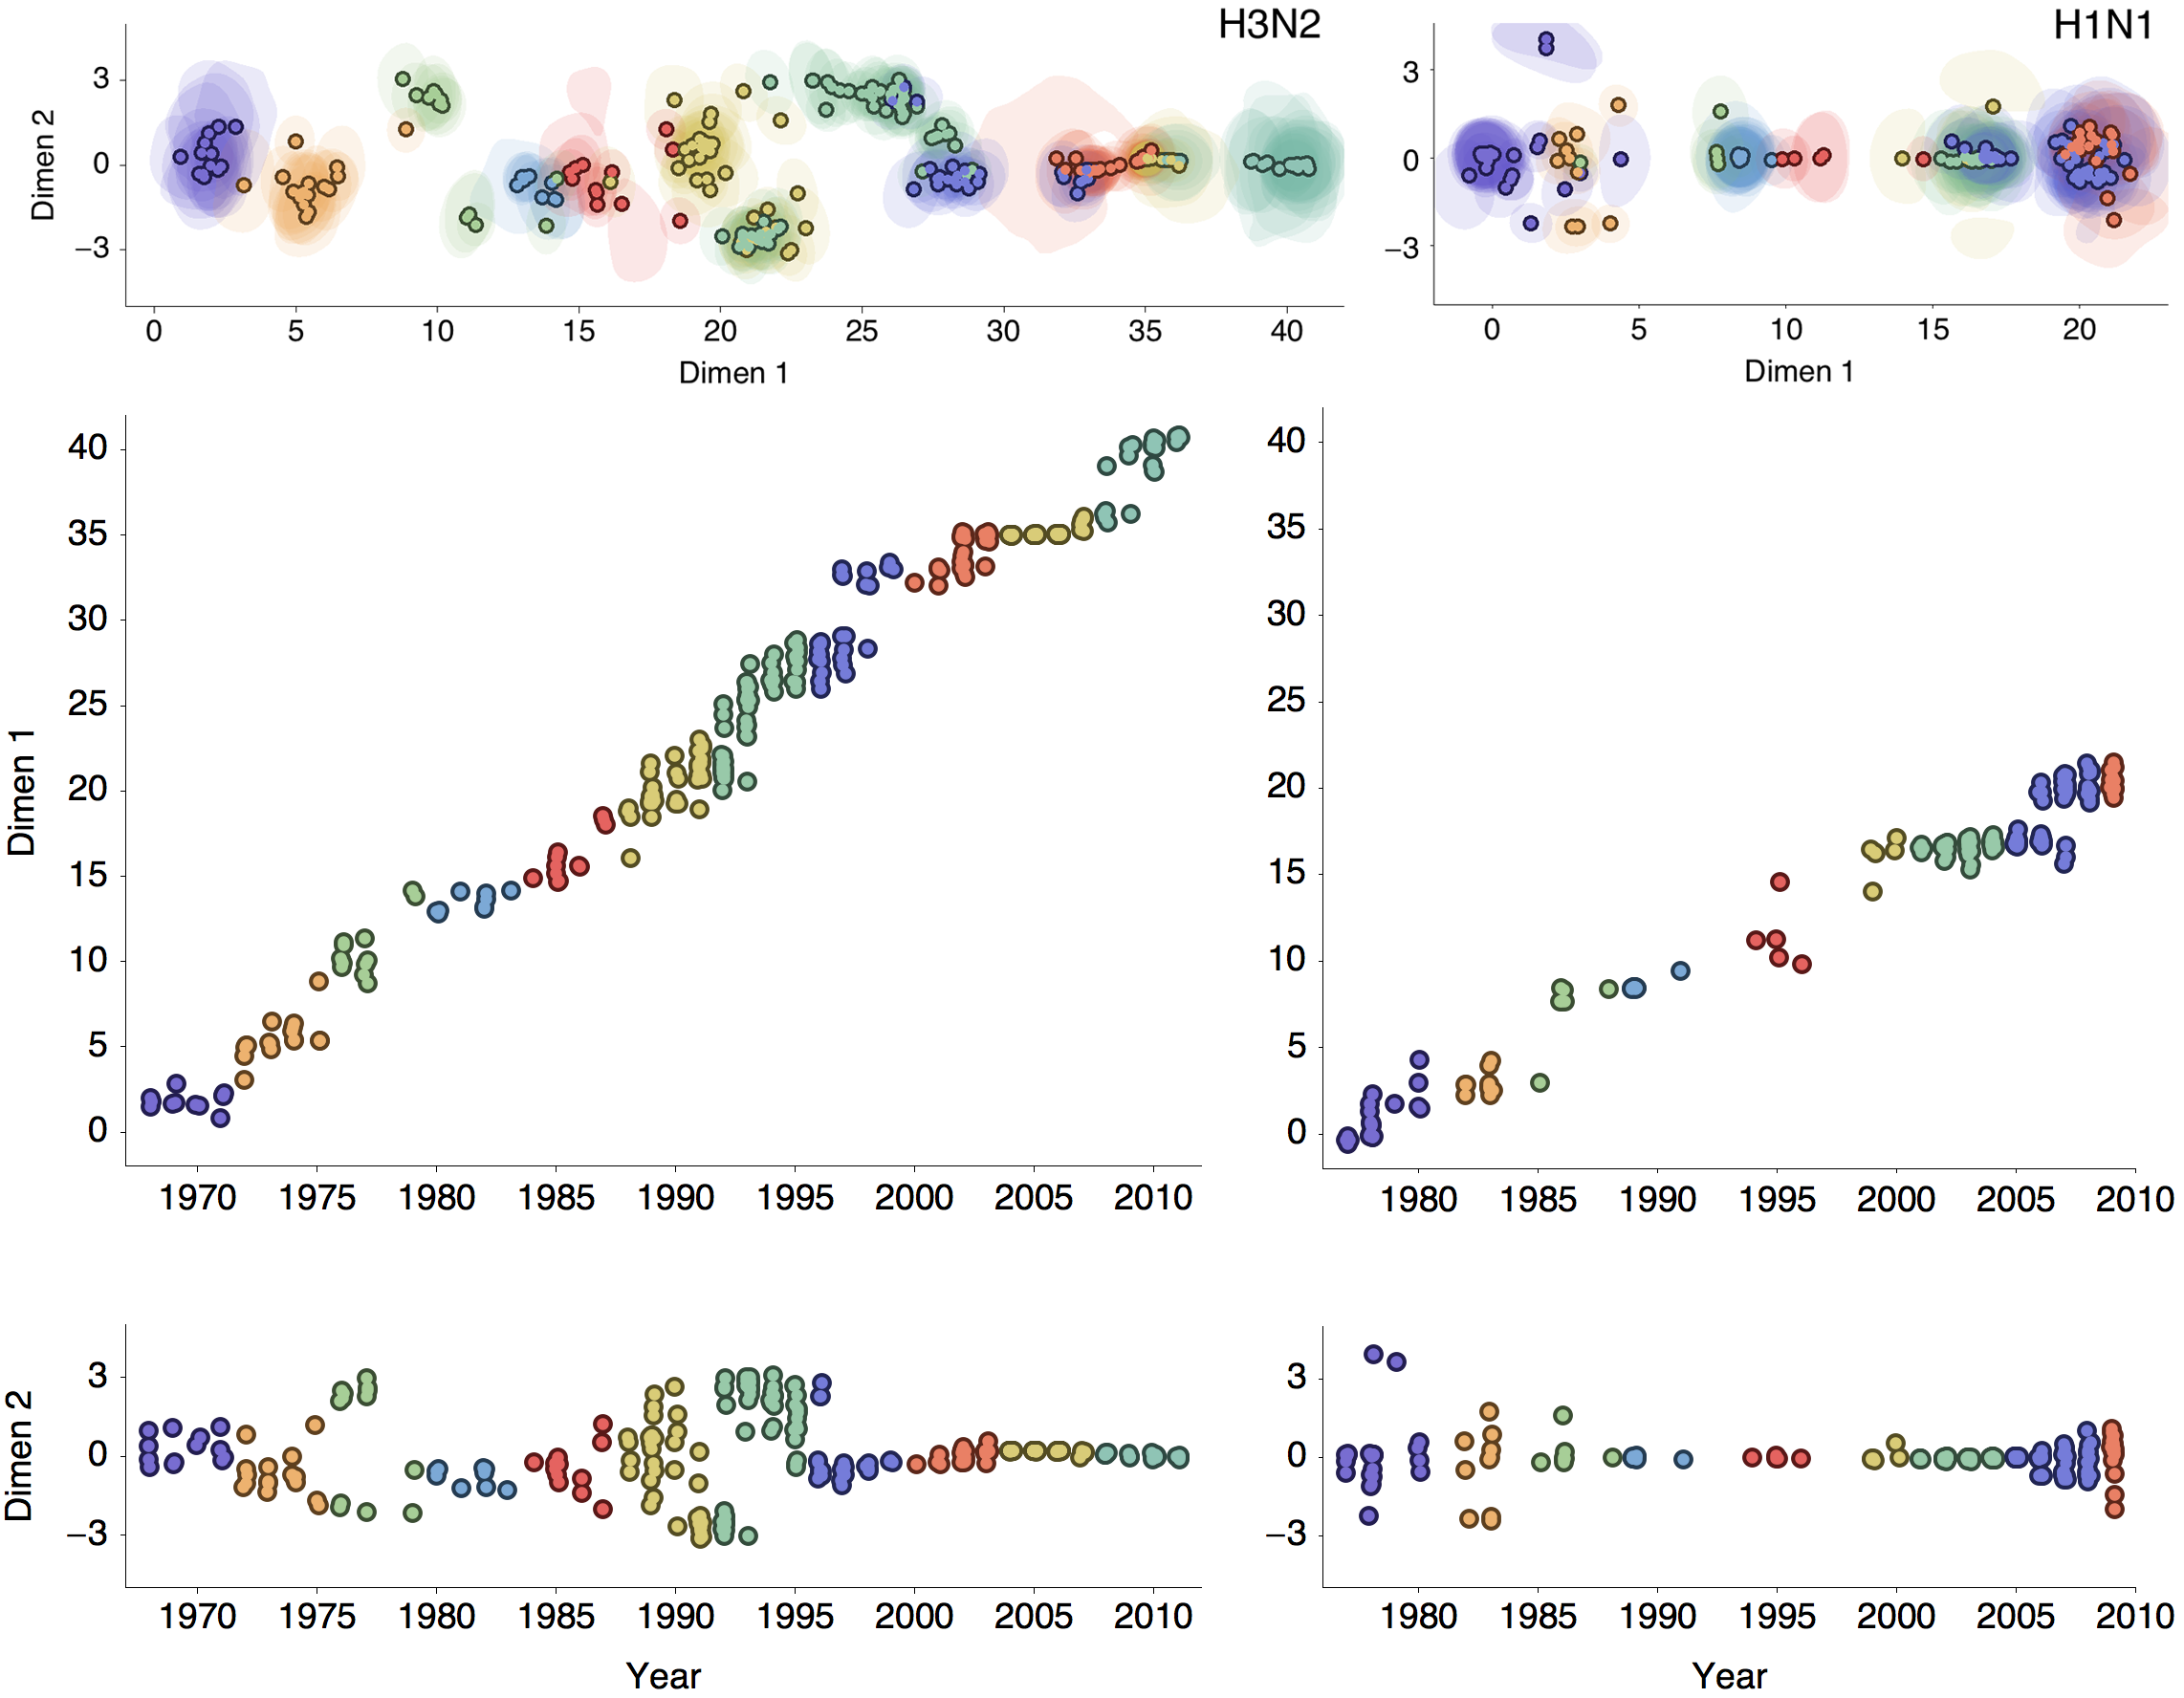
\includegraphics[width=\textwidth]{figures/flu_grid}
	\caption{\textbf{Antigenic locations of influenza H3N2 and H1N1.} 
	(A) and (B) Antigenic maps showing the mean posterior location of 338 strains of H3N2 influenza and 243 strains of H1N1 influenza.  
	The model has been constructed so that the primary axis of variation lies along the $x$-axis (AG1), with the $y$-axis (AG2) orthogonal to this axis.  
	(C) and (D) Antigenic location along the primary axis of variation (AG1) vs.\ year of virus isolation.  
	The dashed lines show the relationship of between time and AG1 with a slope of \tbc{XXX} for H3N2 and \tbc{XXX} for H1N1.  
	(E) and (F) Antigenic location along the secondary axis of variation (AG2) vs.\ year of virus isolation.  
	Points represent median strain locations and translucent areas represent 50\% highest density regions.
	Antigenic units represent two-fold dilutions of the HI assay, and strains have been colored based on year of isolation.} 
	\label{flu_grid} 
\end{figure}

\subsection*{Competition between influenza lineages}

We investigated the relative rates of antigenic evolution in different influenza lineages from 1999 to 2009, finding a general correspondence between antigenic drift along antigenic dimension 1 and relative incidence between influenza A/H3N2, A/H1N1, B/Victoria and B/Yamagata.
From 1999 to 2009, influenza A (H3N2) accounted for the majority of antigenic evolution (51\%), while A/H1N1, B/Victoria and B/Yamagata split the remainder, accounting for 17\%, 18\% and 14\%, respectively.
Similarly, influenza A (H3N2) was responsible for the majority of incidence (54\%) in the USA during this time period.
Influenza A (H1N1) accounted for 23\% of incidence, B/Victoria accounted for 12\% of incidence and B/Yamagata accounted for 10\% of incidence.
These proportions are significantly similar to one another (randomization test $p = 0.010$).


%%% drift_incidence %%%
\begin{figure}[tb]
	\centering		
	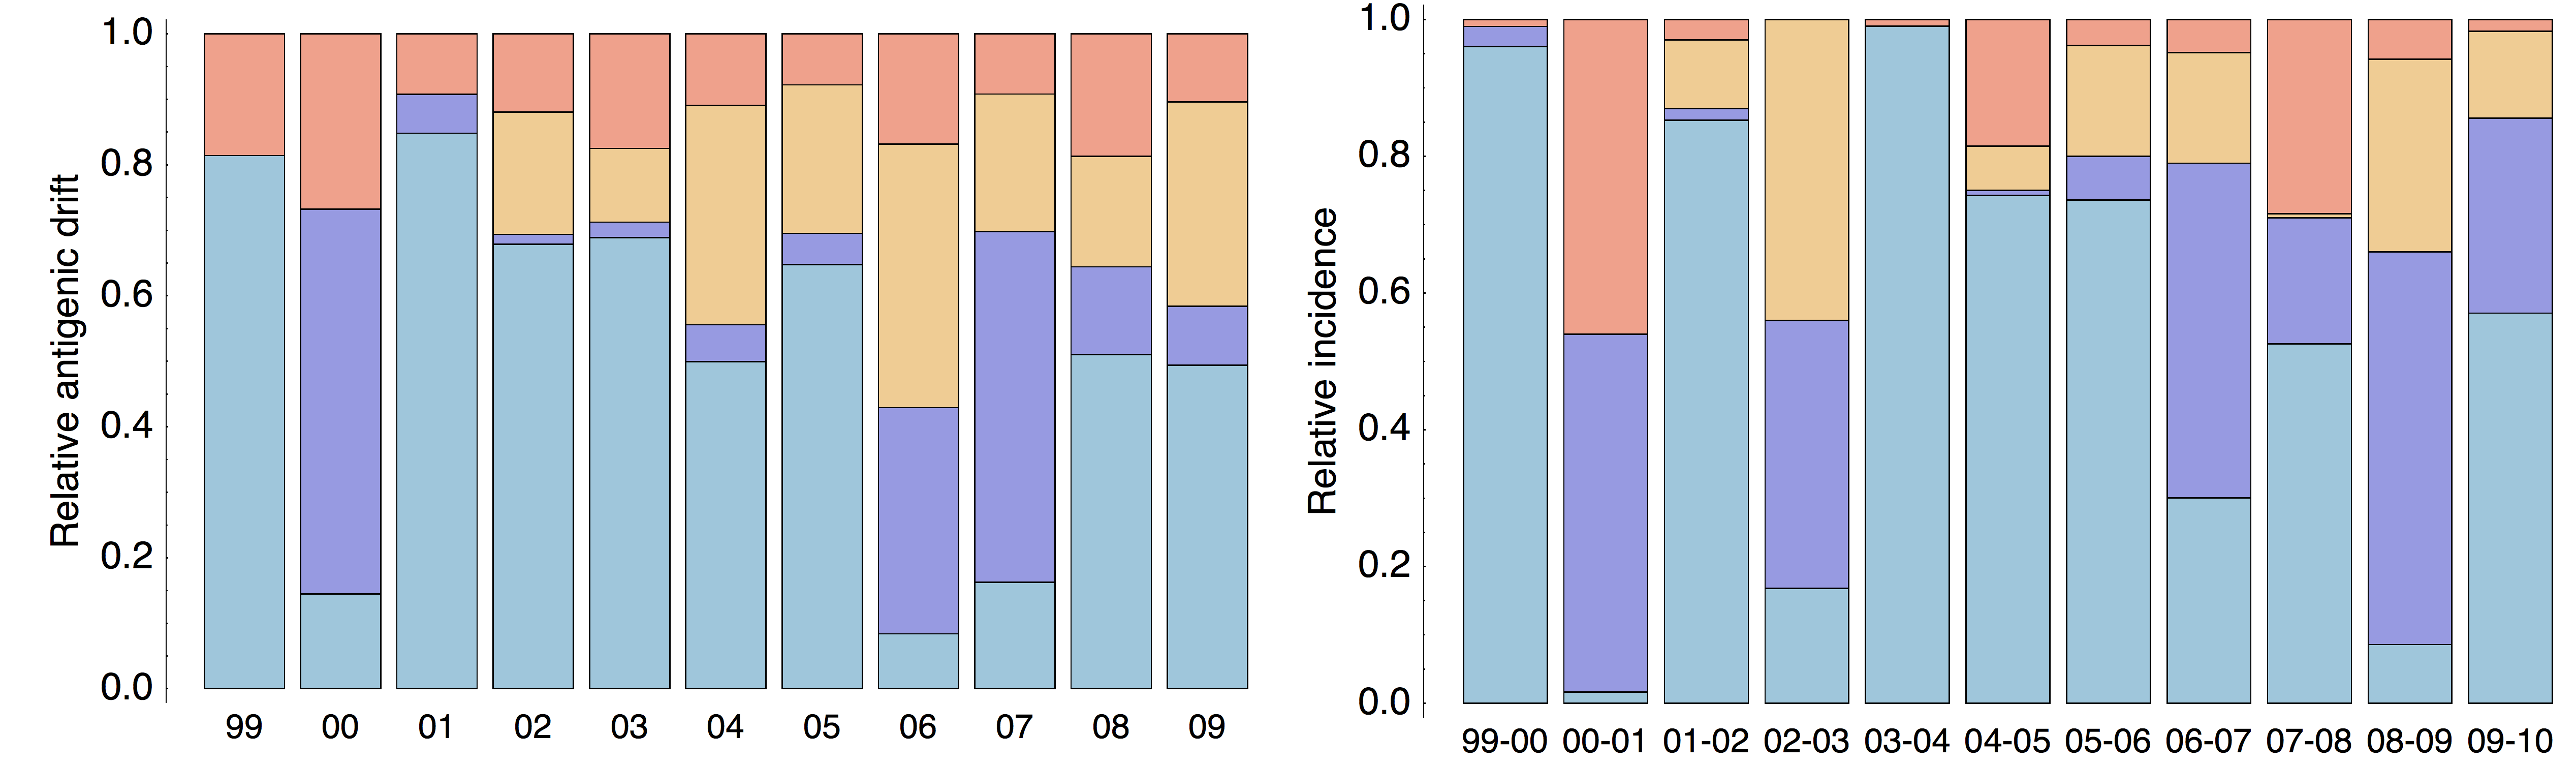
\includegraphics[width=\textwidth]{figures/drift_incidence}
	\caption{\textbf{Relative antigenic drift and incidence between lineages of influenza from 1999 to 2009.} 
	(A) Relative antigenic drift of influenza A H3N2 and H1N1 and influenza B Victoria and Yamagata lineages.
	Relative change in antigenic dimension 1 between year $i$ and year $i-1$ is shown for each of the 4 lineages.
	(B) Relative incidence of influenza A H3N2 and H1N1 and influenza B Victoria and Yamagata lineages.
	Relative isolation counts of each lineage in the USA for each winter influenza season.
	} 
	\label{drift_incidence} 
\end{figure}

%%% DISCUSSION %%%
\section*{Discussion}

%%% METHODS %%%
\section*{Methods}

\subsection*{Genetic and antigenic data}

We compiled an antigenic dataset of hemagglutination inhibition (HI) measurements for influenza A (H3N2) by collecting data from previous publications \cite{Hay01,Smith04,Russell08,Barr10}, NIMR vaccine strain selection reports for 2002 and 2008--2012 \cite{NIMR02,NIMRMarch08,NIMRFeb09,NIMRFeb10,NIMRSep10,NIMRSep11,NIMRFeb12} and the Feb 2011 VRBPAC report \cite{Cox11FDA}.
We queried the Influenza Research Database \cite{IRD} and the EpiFlu Database \cite{GISAID} for HA nucleotide sequences by matching strain names, e.g.\ A/HongKong/1/1968, and only strains for which sequence was present was retained.
If a strain had multiple sequences in the databases we preferentially kept the IRD sequence and preferentially kept the longest sequence in IRD. 
This dataset had 2051 influenza isolates (present as either virus or serum in HI comparisons) dating from 1968 to 2011. 
However, the majority of isolates were present from 2002 to 2007. 
Because we are interested in longer-term antigenic evolution, we censored the data to have at most 20 virus isolates per year, preferentially keeping those isolates with more antigenic comparisons. 
We then kept only those serum isolates that are relatively informative to the antigenic placement of viruses, dropping serum isolates that are compared to 4 or fewer different virus isolates.
This censoring left 429 virus isolates, 519 serum isolates and 10,097 HI measurements. 

Antigenic data for influenza A (H1N1) was collected from previous publications \cite{Kendal78,Webster79,Nakajima79,Nakajima81,Chakraverty82,Pereira82,Chakraverty86,Cox83,Daniels85,Raymond86,Stevens87,Donatelli93,Hay01,Daum02,McDonald07,Barr10} and NIMR vaccine strain selection reports for 2002--2010 \cite{NIMR02,NIMR03,NIMR04,NIMRFeb05,NIMRSep05,NIMRMarch06,NIMRSep06,NIMRMarch07,NIMRSep07,NIMRMarch08,NIMRSep08,NIMRFeb09,NIMRFeb10}.
The same procedure was followed as was followed for H3N2 to match sequence data and to censor antigenic comparisons.
This procedure yielded 124 virus isolates, 77 serum isolates and 1882 HI measurements over the course of 1977 to 2009.

Antigenic comparisons for influenza B Victoria-lineage were collated from previous publications \cite{Hay01} \tbc{Include in BibTex: Ansaldi04, AusWHO06, Barr06, Daum06, Lin07, Muyanga01, Puzelli04, Rota90, Shaw02, Xu04} and NIMR vaccine strain selection reports for 2002--2012 \cite{NIMR02,NIMR03,NIMR04,NIMRFeb05,NIMRSep05,NIMRMarch06,NIMRSep06,NIMRMarch07,NIMRSep07,NIMRMarch08,NIMRFeb09,NIMRSep09,NIMRFeb10,NIMRSep10,NIMRFeb11,NIMRSep11,NIMRFeb12}.
Here, the sequence matching and censoring procedure yielded 179 virus isolates, 70 serum isolates and 2003 HI measurements over the course of 1986 to 2011.

Antigenic comparisons for influenza B Yamagata-lineage were collected from previous publications \cite{Hay01} \tbc{Include in BibTex: Abed03, Ansaldi03, Ansaldi04, AusWHO06, Barr06, Daum06, Kanegae90, Lin07, Matsuzaki04, Muyanga01, Nakagawa02, Nakajima92, Nerome98, Puzelli04, Rota90, Shaw02, Xu04} and NIMR vaccine strain selection reports for 2002--2012 \cite{NIMR02,NIMR03,NIMR04,NIMRFeb05,NIMRSep05,NIMRMarch06,NIMRSep06,NIMRMarch07,NIMRSep07,NIMRMarch08,NIMRFeb09,NIMRSep09,NIMRFeb10,NIMRSep10,NIMRFeb11,NIMRSep11,NIMRFeb12}.
For B/Yamagata, the matching and censoring procedure resulted in 174 virus isolates, 69 serum isolates and 1962 HI measurements over the course of 1987 to 2011.

Sequences were aligned using MUSCLE v3.7 under default parameters \cite{MUSCLE}.

\subsection*{Antigenic cartography and Bayesian multidimensional scaling}

Antigenic characteristics of viral strains are often assessed through immunological assays such as hemagglutination inhibition (HI) \cite{Hirst43}.  
At heart, these assays compare the reactivity $H_{ij}$ of one virus strain $i$ to antibodies raised against another virus strain $j$ via challenge or vaccination.  
In the case of HI, the measurement of cross-reactivity takes the form of a titer representing the dilution factor at which serum raised against virus $j$ ceases to be effective at inhibiting binding of virus $i$.  
These factors are commonly assessed by serial dilution, so that HI titers will form a log series, 40, 80, 160, etc \dots.
However, due to experimental constraints, most comparisons cannot be made, leading to a sparse observation matrix $\mathbf{H} = \{H_{ij}\}$.  
Further, measurements are usually interval and truncated, e.g.\ inhibition or neutralization may cease somewhere between the serial titers of 160 and 320, or inhibition or neutralization may be absent at all titers assayed, suggesting a threshold somewhere between 0 and 40.  

Previous work \cite{Smith04, Cai10} has used multidimensional scaling to place viruses and sera on an `antigenic map'.  
These methods heuristically optimize locations of viruses and sera by seeking to minimize the sum of squared errors between titers predicted by map locations and observed titers.  
Antigenic maps produced by these methods have proved useful in categorizing virus phenotypes \cite{Smith04}, but the extension of these methods to integrate genetic data has not yet been attained.

Here, we follow previous models in representing antigenic locations as points in an $N$-dimensional antigenic map. 
Our goal is to find an optimal projection of the high-dimensional distance matrix $\mathbf{H}$ into a lower number of dimensions. 
We conduct this projection using Bayesian multidimensional scaling (BMDS) \cite{Oh01} in which a probabilistic model is constructed to quantify the fit of a particular configuration of cartographic locations to the observed matrix of serological measurements.

Let $X_i \in \Re^{P}$ represent the cartographic location of virus $i$ for $i = 1,\ldots,\vn$, and $Y_j$ represent the cartographic location of serum $j$ for $j = 1,\ldots,\sn$.
Virus and antiserum may be isolated from / raised against the same strain and have different cartographic locations.
Typically, $P = 2$, but higher or lower dimensions may better reflect the data.  
This gives set of distances between virus and serum cartographic locations 
\begin{equation}
	\delta_{ij} =  || X_i - Y_j ||_2.
\end{equation}
Here, $H_{ij}$ represents the log$_2$ titer of virus $i$ against serum $j$, and immunological distance can be defined as
\begin{equation}
	d_{ij} =  S_j - H_{ij},
\end{equation}
where $S_j = \max ( H_{1j},\ldots,H_{\vn j} )$.
Traditionally, the goal of multidimensional scaling (MDS) optimizes over $\mathbf{X}$ and $\mathbf{Y}$ such that
\begin{equation}
	\sum_{(i,j) \in \cal I} 
	\left(
		\delta_{ij} - d_{ij}
	\right)^2
\end{equation}
is minimized, where $\cal I = \{ (i,j) : H_{ij} \mbox{ is measured} \}$. 
Here, we instead assume a probabilistic interpretation in which an observed titer is normally distributed around its cartographic expectation
\begin{equation} 
	H_{ij} \sim \mbox{Normal}( S_j - \delta_{ij}, \mdssd^2 ),
\end{equation}
and the likelihood of observing a particular titer given the placement of antigenic locations is 
\begin{equation} 
	\point(H_{ij}) = \phi \left( \frac{ H_{ij} + \delta_{ij} - S_j }{ \mdssd } \right),
\end{equation}
where $\mdssd^2$ represents variance and $\phi(\cdot)$ represents the standard normal PDF.
HI assays sometimes show no inhibition at all measured titrations, e.g.\ a measurement can be reported as `$<$40'.
In this case, the likelihood of observing the threshold measurement follows the cumulative density of the lower tail of the normal distribution
\begin{equation} 
	\threshold(H_{ij}) = \Phi \left( \frac{ H_{ij} + \delta_{ij} - S_j }{ \mdssd } \right),
\end{equation}
where $\Phi(\cdot)$ represents the standard normal CDF.
Although it is simplest to assume that immunological measurements represent point estimates, it seems more natural to assume that the threshold for inhibition occurs between two titers, e.g.\ we observe inhibition at 1:40 dilution and no inhibition at 1:80 dilution.
Rather than taking the HI titer as 40, we can instead treat this as an interval measurement, assuming that the exact titer for inhibition would occur somewhere between 40 and 80.
HI titers are usually reported as the highest titer that successfully inhibits virus binding or growth, so that in this case, we calculate the likelihood of an interval measurement as
\begin{equation} 
	\interval(H_{ij}) = \Phi \left( \frac{ H_{ij} + \delta_{ij} - S_j + 1 }{ \mdssd } \right) - \Phi \left( \frac{ H_{ij} + \delta_{ij} - S_j }{\mdssd} \right).
\end{equation}
These likelihoods are illustrated in Figure \ref{hij_likelihood}.
Throughout our analyses, we use interval likelihoods $\interval$ rather than point likelihoods $\point$ unless otherwise noted.

%%% hij_likelihood %%%
\begin{figure}[tb]
	\centering		
	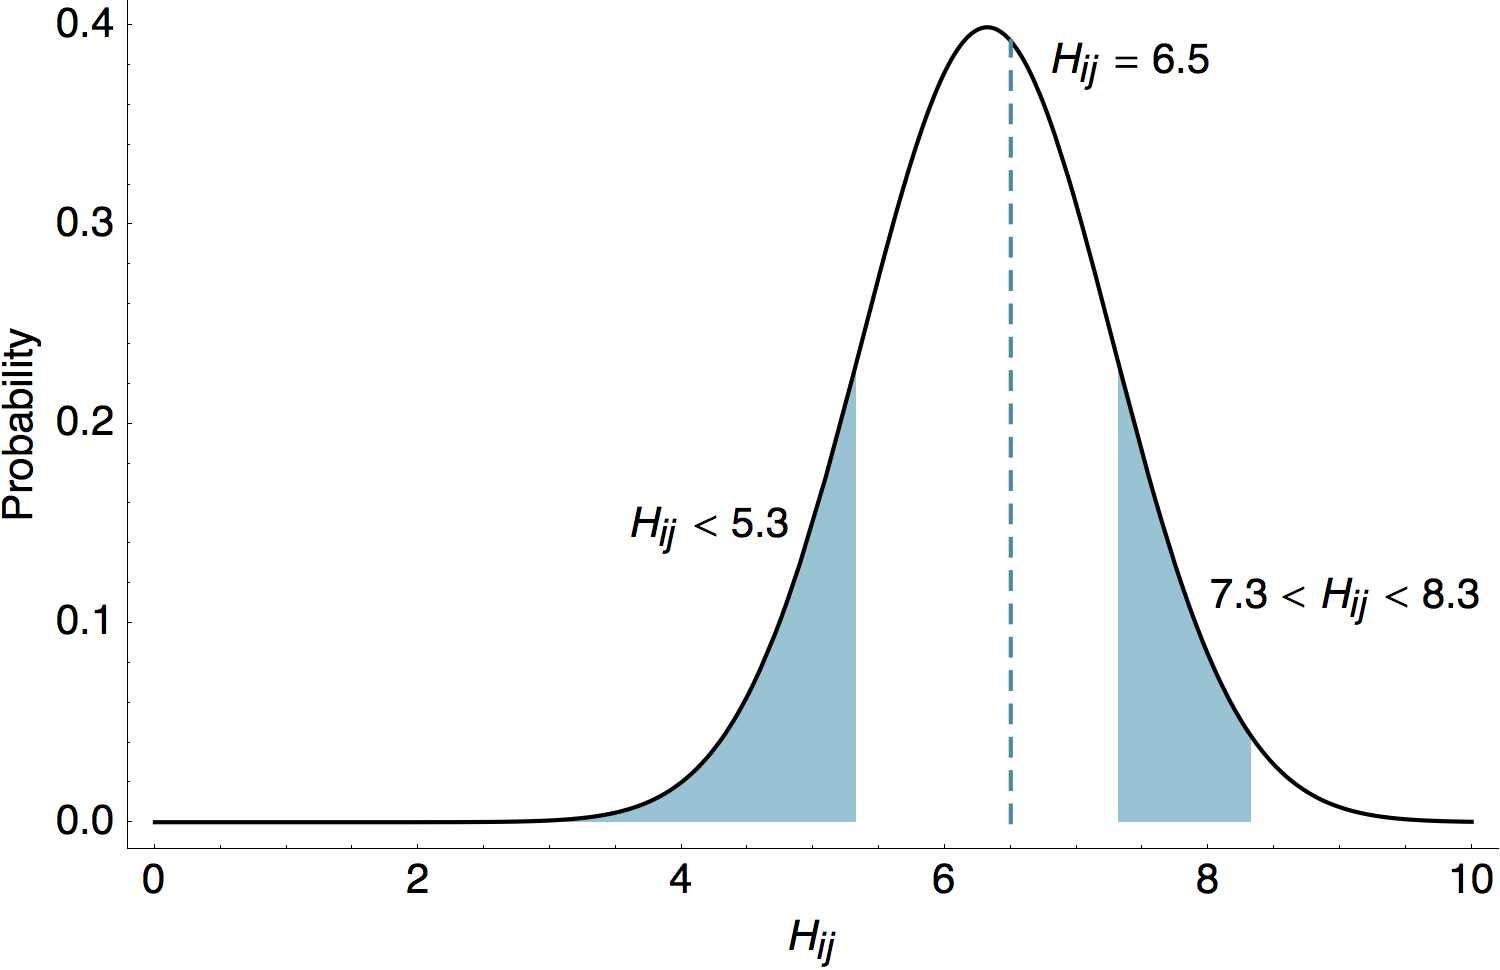
\includegraphics[width=0.6\textwidth]{figures/hij_likelihood}
	\caption{\textbf{Likelihood of HI titers in the BMDS model.} 
	Here we show the likelihoods of observing three different outcomes given $\delta_{ij} = 4$, $\mdssd = 0.95$ and $S_j = \mathrm{log}_2 1280 = 10.32$.  
	The likelihood of observing a threshold titer of `$<$40' is equal to the lower tail of the probability density function $\threshold(5.32) = 0.146$.
	The likelihood of observing a point measurement with an exact inhibiting titer of `90.5' is equal to the density function $\point(6.5) = 0.413$.
	The likelihood of observing an interval measurement with an inhibiting titer somewhere between `160' and `320' is equal to $\interval(7.32) = 0.129.$
	} 
	\label{hij_likelihood} 
\end{figure}

We calculate the overall likelihood by multiplying probabilities of individual measurements
\begin{equation} 
	L(\mathbf{X},\mathbf{Y}) = \prod_{(i,j) \in \cal I} f(H_{ij}),
\end{equation}
using probability functions $\point$, $\threshold$ and $\interval$ as appropriate.
We assume that the prior precision $1/\mdssd^2$ follows a diffuse $\mbox{Gamma}(a, b)$ distribution with $a=0.001$ and $b=1000$, and we start by assuming a uniform prior over virus and sera locations $\mathbf{X}$ and $\mathbf{Y}$.

We integrate over uncertainty using the Markov chain Monte Carlo (MCMC) procedures implemented in the phylogenetic package BEAST \cite{BEAST}.
Metropolis-Hastings proposals include moves to individual virus and serum locations $X_i$ and $Y_j$, scaling of the entire set of virus and serum locations $\mathbf{X}$ and $\mathbf{Y}$ and scaling $\mdssd$.

\subsection*{Incorporating virus and serum effects}

The preceding model represents immunological distance as a drop in titer against the most reactive comparison for a particular antiserum.  
Here, we relax this assumption and treat the maximum reactivity of a sera as a random variable.
In this case, $H_{ij}$ still follows
\begin{equation} 
	H_{ij} \sim \mbox{Normal}( S_j - \delta_{ij}, \mdssd^2 ),
\end{equation}
but the vector of `serum effects' $\mathbf{S}$ is estimated rather than fixed.
We assume that $S_j$ values are hierarchically distributed according to a normal distribution.
The mean and variance of this distribution is taken from the empirical mean and empirical variance of the set of maximum titers across sera $\{ \max ( H_{1j},\ldots,H_{\vn j} ) : j = 1,\ldots,\sn \}$.
This formulation assumes that particular sera are more reactive in general than other sera.

Additionally, we follow the same logic and assume that particular virus isolates are more reactive in general than other virus isolates.
With virus reactivity included, $H_{ij}$ follows
\begin{equation} 
	H_{ij} \sim \mbox{Normal}\left(  \frac{V_i+S_j}{2} - \delta_{ij}, \mdssd^2 \right),
\end{equation}
and the vector of `virus effects' $V_i$ for $i = 1,\ldots, \vn$ is estimated in an analogous hierarchical fashion, with $\mathbf{V}$ normally distributed with mean and variance equal to the empirical mean and variance of the set of maximum titers across viruses $\{ \max ( H_{i1},\ldots,H_{i \sn} ) : i = 1,\ldots,\vn \}$.

With these effects included, Metropolis-Hastings proposals additionally incorporate moves to individual serum effects $S_j$ and virus effects $V_i$.

%%% ACKNOWLEDGMENTS %%%
\subsection*{Acknowledgments} 

%%% FUNDING %%%
\subsection*{Funding} 

%%% REFERENCES %%%
\bibliographystyle{plos}
\bibliography{flux}

\pagebreak

\setcounter{figure}{0}
\setcounter{table}{0}
\setcounter{page}{1}
\renewcommand{\thefigure}{S\arabic{figure}}
\renewcommand{\thetable}{S\arabic{table}}
\renewcommand{\thepage}{S\arabic{page}}

%%% SUPPORTING INFORMATION %%%
\section*{Supporting Information}

\pagebreak

\end{document}
